\documentclass{article}
\usepackage{graphicx} 
\usepackage{amsmath}
\usepackage{gauss, amssymb}
\usepackage{nicematrix}
\usepackage[utf8]{inputenc}
\usepackage[T1]{fontenc}
\usepackage[english]{babel}
\usepackage[nottoc,notlot,notlof]{tocbibind}
\usepackage[hidelinks]{hyperref}
\usepackage{amsthm}
\usepackage{physics}
\usepackage{booktabs}
\usepackage{nicematrix}
\usepackage{tikz}
\usepackage{algorithm2e}
\usetikzlibrary{arrows.meta, positioning, shapes.geometric}

\theoremstyle{definition}
\newtheorem{definition}{Definition}[section]


\newcommand{\mycomment}[1]{}

% Define \circled
\newcommand*\circled[1]{\tikz[baseline=(char.base)]{
            \node[shape=circle,draw,inner sep=1pt] (char) {#1};}}

\title{ - Maskinlæring H25}
\date{\today}
%This material is based upon the book 
\begin{document}

\maketitle

\tableofcontents

\newpage

%\section{Introduction}

\newpage
\section{Statistical Learning}

Statistical learning is concerned with understanding and estimating the relationship between a target variable \( Y \) and one or more predictors \( X = (X_1, X_2, \ldots, X_p) \).  
We typically assume the model:
\[
Y = f(X) + \epsilon
\]
where \( f(X) \) is the systematic part of the relationship, and \( \epsilon \) is random noise with mean zero.

\subsection{Supervised Learning}

In supervised learning, both the predictors \( X \) and the response \( Y \) are observed, and the goal is to estimate the mapping \( f: X \mapsto Y \).

\subsubsection{Types of Supervised Learning}
Depending on the type of \( Y \), we distinguish between:

\begin{center}
\begin{tabular}{@{}lll@{}}
\toprule
Type of \( Y \) & Task & Example \\
\midrule
Continuous (quantitative) & Regression & Predicting sales, temperature, price \\
Discrete (qualitative) & Classification & Predicting spam vs.\ non-spam, disease vs.\ healthy \\
\bottomrule
\end{tabular}
\end{center}

\subsubsection{Example: Predicting Sales}
Suppose we want to predict sales \( Y \) using advertising budgets in three media channels:
\[
X_1 = \text{TV}, \quad X_2 = \text{Radio}, \quad X_3 = \text{Newspaper.}
\]
We assume
\[
Y = f(X_1, X_2, X_3) + \epsilon
\]
and start with a linear model:
\[
f(X) = \beta_0 + \beta_1 X_1 + \beta_2 X_2 + \beta_3 X_3.
\]

\subsubsection{Estimating \( f \) Using Squared Loss}

To estimate \( f \), we minimize the squared loss:
\[
L(y_i, \hat{f}(x_i)) = (y_i - \hat{f}(x_i))^2,
\]
and the total (mean) squared error:
\[
\text{MSE}(\hat{f}) = \frac{1}{n}\sum_{i=1}^{n}(y_i - \hat{f}(x_i))^2.
\]

The optimal parameters \( \beta_j \) are found by minimizing the MSE, leading to the ordinary least squares (OLS) solution:
\[
\hat{\boldsymbol{\beta}} = (X^T X)^{-1} X^T y.
\]

\subsection{Unsupervised Learning}

In unsupervised learning, only the predictors \( X \) are observed; there is no corresponding response variable \( Y \).  
The goal is to discover structure or patterns within the data.

\subsubsection{Clustering}
A common example is \textbf{clustering}, where observations are grouped based on similarity among predictors \( X_1, X_2, \ldots \).  
For instance, clustering points \( (x_1, x_2) \) may reveal natural groupings or clusters within a dataset.

\subsubsection{Outcomes}
In contrast to supervised learning:
\begin{itemize}
    \item Continuous outcomes correspond to \textbf{regression}.
    \item Discrete outcomes correspond to \textbf{classification}.
\end{itemize}

\subsection{Least Squares Regression}

In least squares regression, we assume a model such as:
\[
f(X) = \beta_0 + \beta_1 X_1 + \beta_2 X_1^2,
\]
which can capture some curvature or nonlinearity.

While more flexible models can better fit training data, they also introduce new issues such as \textbf{overfitting}.  
We can measure performance using the Mean Squared Error (MSE):
\[
\text{MSE} = \frac{1}{n}\sum_{i=1}^{n} (y_i - \hat{f}(x_i))^2.
\]

The error can be decomposed into:
\begin{itemize}
    \item \textbf{Training error}: computed on the same data used to fit the model.
    \item \textbf{Test (validation) error}: computed on unseen data.
\end{itemize}

A model that fits the training data too closely may not generalize well to new data this is overfitting.  
The aim is to find a balance between underfitting and overfitting.

As a general rule of thumb, more flexible methods tend to perform better than inflexible ones, but they must be validated using separate \textbf{validation} and \textbf{test} sets.

\subsection{Bias--Variance Tradeoff}

The expected prediction error for a given \( x_0 \) can be decomposed as:
\[
\mathbb{E}\big[(Y - \hat{f}(x_0))^2\big] = 
\big[\text{Bias}(\hat{f}(x_0))\big]^2 + \text{Var}(\hat{f}(x_0)) + \sigma_\epsilon^2,
\]
where:
\begin{itemize}
    \item \( \sigma_\epsilon^2 = \text{Var}(\epsilon) \) is the irreducible error,
    \item \( \text{Bias}(\hat{f}(x_0)) = \mathbb{E}[\hat{f}(x_0)] - f(x_0) \),
    \item \( \text{Var}(\hat{f}(x_0)) \) is the variability of the estimate.
\end{itemize}

We cannot reduce the irreducible error, but we can trade off bias and variance.  
Accuracy depends on finding the right balance:
\begin{itemize}
    \item High bias \(\Rightarrow\) underfitting.
    \item High variance \(\Rightarrow\) overfitting.
\end{itemize}

Interpretability often decreases as model flexibility increases.

\subsection{Classification}

In classification, the goal is to predict a qualitative response \( Y \) taking values in a finite set of classes \( \{1, 2, \ldots, K\} \).

\subsubsection{K-Nearest Neighbours (KNN)}
Given a new observation \( x_0 \), KNN identifies the \( K \) training points closest to \( x_0 \) (denoted \( \mathcal{N}_0 \)) and estimates:
\[
\Pr(Y = j \mid X = x_0) = \frac{1}{K} \sum_{i \in \mathcal{N}_0} I(Y_i = j),
\]
where \( I(\cdot) \) is the indicator function.

The predicted class is:
\[
\hat{y}_0 = \arg\max_j \Pr(Y = j \mid X = x_0).
\]

\subsubsection{Classification Error}
The classification error rate is:
\[
\text{Error} = \frac{1}{K} \sum_{i \in \mathcal{N}_0} I(Y_i \neq \hat{Y}_i).
\]

\subsubsection{Bayes Classifier}
The Bayes classifier assigns each observation to the most probable class:
\[
\hat{y}_{\text{Bayes}} = \arg\max_j \Pr(Y = j \mid X = x),
\]
which theoretically minimizes the classification error.  
In practice, methods like KNN approximate this boundary, sometimes sacrificing perfect classification to reduce noise.

\subsubsection{Key Idea}
A fundamental rule to remember is:
\[
Y = f(X) + \epsilon.
\]
This holds true for both regression and classification settings the goal of statistical learning is to estimate \( f \) as accurately as possible.

 

\newpage
\section{Generative Models}

Generative models aim to model the joint probability distribution \( P(x, y) \) over inputs \( x \) and labels \( y \).  
By Bayes' theorem:
\[
P(x, y) = P(x \mid y) P(y)
\]
They attempt to learn the underlying structure of the data — allowing inference of missing labels, anomaly detection, and generation of new (synthetic) samples.

Given training data:
\[
T = \{ (x_i, y_i) \}_{i=1}^{n}
\]
we aim to generalize from the observed data to find a hypothesis \( h(x) \in \mathcal{H} \) that minimizes a suitable loss function.

---

\subsection{Gaussian Mixture Models (GMMs)}

A \textbf{Gaussian Mixture Model (GMM)} assumes that the data are generated from a mixture of \( K \) Gaussian distributions:
\[
P(x) = \sum_{k=1}^{K} \pi_k \, \mathcal{N}(x \mid \mu_k, \Sigma_k)
\]
where:
\begin{itemize}
    \item \( \pi_k \) is the mixture coefficient (\( \sum_k \pi_k = 1 \)),
    \item \( \mu_k \) is the mean of cluster \( k \),
    \item \( \Sigma_k \) is the covariance of cluster \( k \),
    \item \( \mathcal{N}(x \mid \mu_k, \Sigma_k) \) is the multivariate Gaussian PDF.
\end{itemize}

Each class or cluster is represented as a multivariate Gaussian distribution.  
The model can describe both separate and overlapping clusters, as shown below.

\begin{figure}[h]
\centering
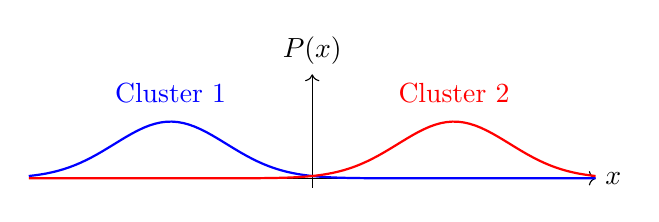
\begin{tikzpicture}[scale=1.2]
% Axes
\draw[->] (-3,0) -- (3,0) node[right] {$x$};
\draw[->] (0,-0.1) -- (0,1.1) node[above] {$P(x)$};

% Two Gaussian curves
\draw[thick,blue,domain=-3:3,samples=100] 
  plot (\x,{0.6*exp(-(\x+1.5)^2/0.7)});
\draw[thick,red,domain=-3:3,samples=100] 
  plot (\x,{0.6*exp(-(\x-1.5)^2/0.7)});

% Labels
\node[blue] at (-1.5,0.9) {Cluster 1};
\node[red] at (1.5,0.9) {Cluster 2};
\end{tikzpicture}
\caption{Two clusters represented by Gaussian components in a GMM. Overlap between clusters indicates probabilistic (soft) boundaries.}
\end{figure}

---

\subsection{Supervised, Unsupervised, and Semi-supervised Learning}

GMMs and K-Means can both be used for clustering:

\begin{itemize}
    \item \textbf{K-Means:} hard assignments — each point belongs to one cluster.
    \item \textbf{GMM:} soft assignments — each point has a probability of belonging to each cluster.
\end{itemize}

\textbf{GMMs can be used for:}
\begin{itemize}
    \item \textbf{Unsupervised learning:} to discover latent clusters in unlabeled data.
    \item \textbf{Supervised learning:} to estimate class-conditional distributions \( P(x \mid y) \).
    \item \textbf{Semi-supervised learning:} to combine labeled and unlabeled data.
\end{itemize}

\textbf{Semi-supervised GMM Algorithm:}
\begin{enumerate}
    \item Learn the initial GMM from available (labeled + unlabeled) data.
    \item Predict missing labels using the current model (e.g., via QDA or posterior probability).
    \item Update the GMM using all data (including predicted labels).
    \item Repeat until convergence (the loss no longer decreases).
\end{enumerate}

\begin{figure}[h]
\centering
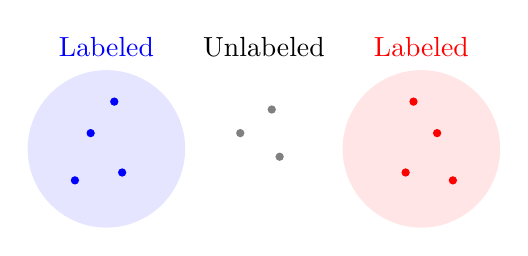
\begin{tikzpicture}[scale=1.0]
% Two clusters
\fill[blue!20,opacity=0.5] (-2,0) circle (1);
\fill[red!20,opacity=0.5] (2,0) circle (1);
% Points
\foreach \x/\y in {-2.2/0.2, -1.8/-0.3, -2.4/-0.4, -1.9/0.6} {
  \fill[blue] (\x,\y) circle (1.5pt);
}
\foreach \x/\y in {2.2/0.2, 1.8/-0.3, 1.9/0.6, 2.4/-0.4} {
  \fill[red] (\x,\y) circle (1.5pt);
}
% Unlabeled
\foreach \x/\y in {-0.3/0.2, 0.2/-0.1, 0.1/0.5} {
  \fill[gray] (\x,\y) circle (1.5pt);
}
\node at (-2,1.3) {\textcolor{blue}{Labeled}};
\node at (2,1.3) {\textcolor{red}{Labeled}};
\node at (0,1.3) {Unlabeled};
\end{tikzpicture}
\caption{Semi-supervised data distribution: labeled and unlabeled points.}
\end{figure}

---

\subsection{Choosing the Number of Clusters (Elbow Method)}

The \textbf{elbow method} is used to select the optimal number of clusters \( K \). It plots the within-cluster sum of squares (WCSS) versus \( K \).  
The ``elbow'' point indicates where adding more clusters provides diminishing returns.

\begin{figure}[h]
\centering
\begin{tikzpicture}[scale=1.0]
% Axes
\draw[->] (0,0) -- (5,0) node[right] {$K$};
\draw[->] (0,0) -- (0,3.2) node[above] {WCSS};
% Curve
\draw[thick,blue,domain=1:4.5,smooth] plot (\x,{3/(0.8*\x+0.5)+0.2});
% Dots
\foreach \x in {1,2,3,4} {
  \fill[blue] (\x,{3/(0.8*\x+0.5)+0.2}) circle (1.5pt);
}
\node[above right,blue] at (2,1.9) {Elbow point};
\draw[dashed] (2,0) -- (2,2);
\end{tikzpicture}
\caption{Elbow method: the optimal $K$ occurs at the elbow point where reduction in error slows down.}
\end{figure}

---

\subsection{Anomaly Detection with GMMs}

GMMs can detect anomalies by identifying points with very low probability density.

Let \( P(x_{\text{test}}) \) be the probability density of a test observation.  
If
\[
P(x_{\text{test}}) < \epsilon
\]
for some threshold \( \epsilon \), the observation is classified as an \textbf{anomaly}.

\textbf{Applications:}
\begin{itemize}
    \item Fraud detection (e.g., credit card transactions)
    \item Aircraft health monitoring (heat, vibration)
    \item Data center metrics:
    \begin{itemize}
        \item \( x_1 \): memory usage
        \item \( x_2 \): disk space
        \item \( x_3 \): CPU load
        \item \( x_4 \): network traffic
    \end{itemize}
\end{itemize}

\begin{figure}[h]
\centering
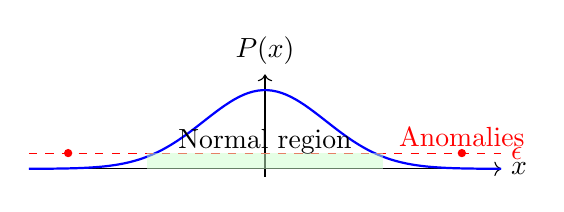
\begin{tikzpicture}[scale=1.0]
% Axes
\draw[->] (-3,0) -- (3,0) node[right] {$x$};
\draw[->] (0,-0.1) -- (0,1.2) node[above] {$P(x)$};

% Gaussian
\draw[thick,blue,domain=-3:3,samples=100] plot (\x,{exp(-(\x)^2/1.2)});
% Threshold
\draw[dashed,red] (-3,0.2) -- (3,0.2) node[right] {$\epsilon$};
% Normal region
\fill[green!20,opacity=0.5] (-1.5,0) rectangle (1.5,0.2);
\node at (0,0.35) {Normal region};
% Anomalies
\fill[red] (-2.5,0.2) circle (1.5pt);
\fill[red] (2.5,0.2) circle (1.5pt);
\node[red] at (2.5,0.4) {Anomalies};
\end{tikzpicture}
\caption{Anomaly detection using GMM: data points below the probability threshold $\epsilon$ are marked as anomalies.}
\end{figure}

---

\subsection{Synthetic Data Generation}

Generative models can also create new synthetic data points from the learned distribution \( P(x) \).  
This can enhance model performance when labeled data are scarce, helping improve cluster separation and classification accuracy.

---

\subsection{Summary and Exam Notes}

\begin{itemize}
    \item Generative models learn \( P(x, y) = P(x \mid y) P(y) \).
    \item GMMs assume data are generated from a mixture of Gaussians.
    \item GMMs can be used for supervised, unsupervised, and semi-supervised learning.
    \item Use the elbow method to determine the number of clusters.
    \item Anomalies are detected when \( P(x_{\text{test}}) < \epsilon \).
    \item Example question: \textit{``What method can handle semi-supervised data?''} → \textbf{GMM (Gaussian Mixture Model)}.
\end{itemize}

\newpage

\end{document}
